\documentclass[12pt]{article}
\usepackage[utf8]{inputenc}
\usepackage{graphicx}
\usepackage[a4paper,width=200mm,top=25mm,bottom=25mm]{geometry}

\title{
{
\includegraphics[width=12cm, height=10cm]{images/csedu_logo.png}}\\
{\large Department of Computer Science and Engineering,\\      University of Dhaka}\\
{ Lab Report for Lab 3 }
}



\author{ Submitted by: Prothito Shovon Majumder \\ Submitted to: Dr. Upama Kabir }



\begin{document}
\maketitle

\newpage
\section{Peripheral Clock Configuration}

\subsection{List of clock registers and their respective purpose:}

\begin{enumerate}
    \item \textbf{RCC clock control register (RCC\_CR)}
    \\ The clock control register RCC\_CR will be used to enable and select the clock source. We can toggle the enable bits to enable PLLSAI, PLLI2S, Main PLL, HSE clock bypass, HSE clock, IHS clock and lock/unlock various ready flags.
    \item \textbf{RCC PLL configuration register (RCC\_PLLCFGR)}
    \\ This register is used to configure the PLL clock outputs according to the formulas.
        \begin{itemize}
            \item f\textsubscript{(VCO clock)} = f\textsubscript{(PLL clock input)} × (PLLN / PLLM)
            \item f\textsubscript{(PLL general clock output)} = f\textsubscript{(VCO clock)} / PLLP
            \item f\textsubscript{(USB OTG FS, SDIO)} = f\textsubscript{(VCO clock)} / PLLQ
        \end{itemize}
    \item \textbf{RCC clock configuration register (RCC\_CFGR)}
    \\  Clock configuration register RCC\_CFGR is used to configure the final bus frequencies. 
    \item\textbf{RCC clock interrupt register (RCC\_CIR)}
    \\ This register is used to configure/enable interrupt flags. We can set the interrupt flags by toggling the corresponding bits to clear/not cleared.
    \item\textbf{RCC AHB1 peripheral reset register (RCC\_AHB1RSTR)}
    \\ The Peripheral Reset Registers should cause the AHB1 peripheral's entire register set and internal state to be reset to it's power-on defaults. This means not just the registers that are exposed to the user, but also any internal registers, counters, or flags should be set as they would be when the device is initially powered on.
    \item\textbf{RCC AHB2 peripheral reset register (RCC\_AHB2RSTR)}
    \\ Just like the prior description of the AHB1 reset register, this reset register is used to cause the state of entire register set and internal state to be reset to it's power-on defaults.
    \item\textbf{RCC AHB3 peripheral reset register (RCC\_AHB3RSTR)}    
    \\ Just like the prior description of the AHB1 reset register, this reset register is used to cause the state of entire register set and internal state to be reset to it's power-on defaults.
    \item\textbf{RCC APB1 peripheral reset register (RCC\_APB1RSTR)}
    \\ Just like the prior description of the AHB1 reset register, this reset register is used to cause the state of entire register set and internal state to be reset to it's power-on defaults.
    \item\textbf{RCC APB2 peripheral reset register (RCC\_APB2RSTR)}
    \\ Just like the prior description of the AHB1 reset register, this reset register is used to cause the state of entire register set and internal state to be reset to it's power-on defaults.
    \item \textbf{RCC AHB1 peripheral clock enable register (RCC\_AHB1ENR) }
    \\ Used to enable and disable bits to control the clocks for various GPIO ports associated with AHB1.
    \item \textbf{RCC AHB2 peripheral clock enable register (RCC\_AHB2ENR) }
    \\ Used to enable and disable bits to control the clocks for various GPIO ports associated with AHB2.
    \item \textbf{RCC AHB3 peripheral clock enable register (RCC\_AHB3ENR) }
    \\ Used to enable and disable bits to control the clocks for various GPIO ports associated with AHB3.
    \item \textbf{RCC APB1 peripheral clock enable register (RCC\_APB1ENR) }
    \\ Used to enable and disable bits to control the clocks for various GPIO ports associated with APB1.
    \item \textbf{RCC APB2 peripheral clock enable register (RCC\_APB2ENR) }
    \\ Used to enable and disable bits to control the clocks for various GPIO ports associated with APB2.
    \item \textbf{RCC AHB1 peripheral clock enable in low power mode register (RCC\_AHB1LPENR)}
    \\ Used to enable or disable the AHB1 peripheral clock during Low Power (Sleep) mode.
    \item \textbf{RCC AHB2 peripheral clock enable in low power mode register (RCC\_AHB2LPENR)}
    \\ Used to enable or disable the AHB2 peripheral clock during Low Power (Sleep) mode.
    \item \textbf{RCC AHB3 peripheral clock enable in low power mode register (RCC\_AHB3LPENR)}
    \\ Used to enable or disable the AHB3 peripheral clock during Low Power (Sleep) mode.
    \item \textbf{RCC APB1 peripheral clock enable in low power mode register (RCC\_APB1LPENR)}
    \\ Used to enable or disable the APB1 peripheral clock during Low Power (Sleep) mode.
    \item \textbf{RCC APB2 peripheral clock enable in low power mode register (RCC\_APB2LPENR)}
    \\ Used to enable or disable the APB2 peripheral clock during Low Power (Sleep) mode.
    \item \textbf{RCC Backup domain control register (RCC\_BDCR)}
        \\ This register is for performing a backup domain reset, handling the real-time clock and the LSE clock.
    \item \textbf{RCC clock control \& status register (RCC\_CSR)}
        \\ This register is mainly used by the hardware to set flags after various resets occur. Software may write to the RMVF bit to clear all reset bits set by hardware.
    \item \textbf{RCC spread spectrum clock generation register (RC\_SSCGR)}
        \\ This register is used for spread spectrum clock generation for the main PLL. It has to be written to before the main PLL is enabled or after the main PLL is disabled.
    \item \textbf{RCC PLLI2S configuration register (RCC\_PLLI2SCFGR)}
        \\ This register is used to configure the PLLI2S clock outputs according to the formulas:
        \begin{itemize}
            \item f\textsubscript{(VCO clock)} = f\textsubscript{(PLLI2S clock input)} × (PLLI2SN / PLLI2SM)
            \item f\textsubscript{(PLL I2S clock output)} = f\textsubscript{(VCO clock)} / PLLI2SR
            \item f\textsubscript{(PLL SPDIFRX clock output)} = f\textsubscript{(VCO clock)} / PLLI2SP
        \end{itemize}
    \item \textbf{RCC PLL configuration register (RCC\_PLLSAICFGR)}
        \\ This register is used to configure the PLLSAI clock outputs according to the formulas:
        \begin{itemize}
            \item f\textsubscript{(VCO clock)} = f\textsubscript{(PLLSAI clock input)} × (PLLSAIN / PLLM)
            \item f\textsubscript{(PLL SAI 48MHz clock output)} = f\textsubscript{(VCO clock)} / PLLSAIP
            \item f\textsubscript{(PLL SAI1 clock output)} = f\textsubscript{(VCO clock)} / PLLSAIQ
        \end{itemize}
    \item \textbf{RCC Dedicated Clock Configuration Register (RCC\_DCKCFGR)}
        \\ This register allows to configure the timer clock prescalers and the PLLSAI and PLLI2S output clock dividers for SAIs peripherals according to the following formula:
        \begin{itemize}
            \item f\textsubscript{(PLLSAIDIVQ clock output)} = f\textsubscript{(PLLSAI\_Q)} / PLLSAIDIVQ
            \item f\textsubscript{(PLLI2SDIVQ clock output)} = f\textsubscript{(PLLI2S\_Q)} / PLLI2SDIVQ
        \end{itemize}
    \item \textbf{RCC clocks gated enable register (CKGATENR)}
        \\ This register allows to enable or disable the clock gating for the specified IPs.
    \item \textbf{RCC dedicated clocks configuration register 2 (DCKCFGR2)}
        \\ This register allows to enable or disable the clock gating for the specified IPs.
\end{enumerate}
\subsection{Memory Address of Clock Registers}
\begin{tabular}{ |c|c| }
        \hline
        \textbf{Clock Register} & \textbf{Memory Address} \\
        \hline
        RCC clock control register (RCC\_CR) & 0x40023800 \\
        \hline
        RCC PLL configuration register (RCC\_PLLCFGR) & 0x40023804 \\
        \hline
        RCC clock configuration register (RCC\_CFGR) & 0x40023808 \\
        \hline
        RCC clock interrupt register (RCC\_CIR) & 0x4002380C \\
        \hline
        RCC AHB1 peripheral reset register (RCC\_AHB1RSTR) & 0x40023810 \\
        \hline
        RCC AHB2 peripheral reset register (RCC\_AHB2RSTR) & 0x40023814 \\
        \hline
        RCC AHB3 peripheral reset register (RCC\_AHB3RSTR) & 0x40023818 \\
        \hline
        RCC APB1 peripheral reset register (RCC\_APB1RSTR) & 0x40023820 \\
        \hline
        RCC APB2 peripheral reset register (RCC\_APB2RSTR) & 0x40023824 \\
        \hline
        RCC AHB1 peripheral clock enable register (RCC\_AHB1ENR)  & 0x40023830 \\
        \hline
        RCC AHB2 peripheral clock enable register (RCC\_AHB2ENR) & 0x40023834 \\
        \hline
        RCC AHB3 peripheral clock enable register (RCC\_AHB3ENR) & 0x40023838 \\
        \hline
        RCC APB1 peripheral clock enable register (RCC\_APB1ENR) & 0x40023840 \\
        \hline
        RCC APB2 peripheral clock enable register (RCC\_APB2ENR) & 0x40023844 \\
        \hline
        RCC AHB1 peripheral clock enable in low power mode register (RCC\_AHB1LPENR) & 0x40023850 \\
        \hline
        RCC AHB2 peripheral clock enable in low power mode register (RCC\_AHB2LPENR) & 0x40023854 \\
        \hline
        RCC AHB3 peripheral clock enable in low power mode register (RCC\_AHB3LPENR) & 0x40023858 \\
        \hline
        RCC APB1 peripheral clock enable in low power mode register (RCC\_APB1LPENR) & 0x40023860 \\
        \hline
        RCC APB2 peripheral clock enable in low power mode register (RCC\_APB2LPENR) & 0x40023864 \\
        \hline
        RCC Backup domain control register (RCC\_BDCR) & 0x40023870 \\
        \hline
        RCC clock control \& status register (RCC\_CSR) & 0x40023874 \\
        \hline
        RCC spread spectrum clock generation register (RC\_SSCGR) & 0x40023880 \\
        \hline
        RCC PLLI2S configuration register (RCC\_PLLI2SCFGR) & 0x40023884 \\
        \hline
        RCC PLL configuration register (RCC\_PLLSAICFGR) & 0x40023888 \\
        \hline
        RCC Dedicated Clock Configuration Register (RCC\_DCKCFGR) & 0x4002388C \\
        \hline
        RCC clocks gated enable register (CKGATENR) & 0x40023890 \\
        \hline
        RCC dedicated clocks configuration register 2 (DCKCFGR2) & 0x40023894 \\
        \hline
    \end{tabular}
\pagebreak
\section{General Purpose Input/Output Registers}
\subsection{List of GPIO registers and their respective purpose:}
\begin{enumerate}
    \item \textbf{GPIO port mode register (GPIOx\_MODER), (x = A..H)}), 
    \par These bits are written by software to configure the I/O direction mode. These modes are: Input mode, General purpose output mode, Alternative function mode, Analog mode.
    \item \textbf{GPIO port output type register (GPIOx\_OTYPER), (x = A..H)}
    \par These bits are written by software to configure the output type of the I/O port.
    \item \textbf{GPIO port output speed register (GPIOx\_OSPEEDR), (x = A..H)}, 
    \par These bits are written by software to configure the I/O output speed. The slew rate, or the pace at which a signal can vary from low to high values (the "rise time" and "fall time"), is controlled by the GPIO speed register. We can increase the rate of change of the output voltage by increasing the GPIO speed (reducing rise time). However, when the GPIO speed grows, so does the circuit's power consumption and noise output. Unless there is a compelling reason to increase GPIO speed, we keep it modest by default.
    \item \textbf{GPIO port pull-up/pull-down register (GPIOx\_PUPDR), (x = A..H)}
    \par These bits are written by software to configure the I/O pull-up or pull-down.
    \item \textbf{GPIO port input data register (GPIOx\_IDR), (x = A..H)}
    \\ These bits are read-only and can be accessed in word mode only. They contain the input value of the corresponding I/O port.
    \item \textbf{GPIO port output data register (GPIOx\_ODR), (x = A..H)}
    \\ These bits can be read and written by software. For atomic bit set/reset, the ODR bits can be individually set and reset by writing to the GPIOx\_BSRR register (x = A..H).
   \\ We can configure the output value of the port using this register. This is used when we want to output a word.
   \item \textbf{GPIO port bit set/reset register (GPIOx\_BSRR), (x = A..H)}
   \\These bits are write-only and can be accessed in word, half-word or byte mode. A read to these bits returns the value 0x0000. 
   \\This and the GPIO port output data register (GPIOx\_ODR) essentially does the same job. But in GPIOx\_ODR, we can write the output word on it, and it will be sent. But the GPIOx\_BSRR register is for more atomic control of the same thing.
   \item \textbf{GPIO port configuration lock register (GPIOx\_LCKR) (x = A..H)}
    \\ This register is used to lock the configuration of the port bits when a correct write sequence is applied to bit 16 (LCKK). The value of bits [15:0] is used to lock the configuration of the GPIO.
    \item \textbf{GPIO alternate function low register (GPIOx\_AFRL) (x = A..H)}
    \\ These bits are written by software to configure alternate function I/Os.
    \item \textbf{GPIO alternate function high register (GPIOx\_AFRH) (x = A..H)}
    \\ These bits are written by software to configure alternate function I/Os.
\end{enumerate}
\subsection{Memory Addresses of GPIO Registers}
\begin{tabular}{ |c|c|c| }
    \hline
    \textbf{GPIOx} & \textbf{Start Addr.} & \textbf{End Addr.} \\
    \hline
    GPIOA & 0x4002 1C00 & 0x4002 1FFF \\
    \hline
    GPIOB & 0x4002 0400 & 0x4002 07FF \\
    \hline
    GPIOC & 0x4002 0800 & 0x4002 0BFF \\
    \hline
    GPIOD & 0x4002 0C00 & 0x4002 0FFF \\
    \hline
    GPIOE & 0x4002 1000 & 0x4002 13FF \\
    \hline
    GPIOF & 0x4002 1400 & 0x4002 17FF \\
    \hline
    GPIOG & 0x4002 1800 & 0x4002 1BFF \\
    \hline
    GPIOH & 0x4002 1C00 & 0x4002 1FFF \\
    \hline
\end{tabular}
\pagebreak
\section{Task iii}
\subsection{Explanation of Code:}
For \verb|AND|, \verb|OR| and \verb|XOR|, the \verb|AND|, \verb|OR| and \verb|EOR| instructions have been used to store the results of bitwise operations of two registers in other registers. \\
FOR \verb|NAND|, \verb|NOR| and \verb|XNOR|, the results of \verb|AND|, \verb|OR| and \verb|XOR| have been \verb|XOR|ed with 0xFFFFFFFF respectively. \\
In case of 16 bits, we set the upper 16 bits of the result to zero using the \verb|MOVT| instruction. For storing constants, we use \verb|MOVW| instruction for 16 bits and \verb|MOV32| instruction for 32 bits.
\subsection{Description of Instructions:}
\textbf{MOVW}\\The \verb|MOVW| instruction only allows \#imm16 values to be loaded into the registers. \\
\textbf{AND}\\The \verb|AND| instruction performs bitwise \verb|AND| operations on the values in Rn and Operand2. \\
\verb|AND{S}{cond} Rd, Rn, Operand2|
\\
\textbf{ORR}\\The \verb|ORR| instruction performs bitwise \verb|ORR| operations on the values in Rn and Operand2.\\
\verb|ORR{S}{cond} Rd, Rn, Operand2|
\\
\textbf{EOR}\\The \verb|EOR| instruction performs bitwise Exclusive OR operations on the values in Rn and Operand2.\\
\verb|EOR{S}{cond} Rd, Rn, Operand2|
\\
\textbf{MOVT}\\ \verb|MOVT| writes \#imm16 to \verb|Rd[31:16]|, without affecting \verb|Rd[15:0]|. You can generate any 32-bit immediate with a \verb|MOV|, \verb|MOVT| instruction pair. The assembler implements the \verb|MOV32| pseudo-instruction for convenient generation of this instruction pair.\\
\textbf{MOV32} \\ The \verb|MOV32| instruction loads a register with either a 32-bit immediate value or any address.\\
\verb|MOVT{cond} Rd, #imm16|\\
\pagebreak
\subsection{Screenshot of the System State after Loading the Code:}
\begin{figure}[ht]
    \centering
    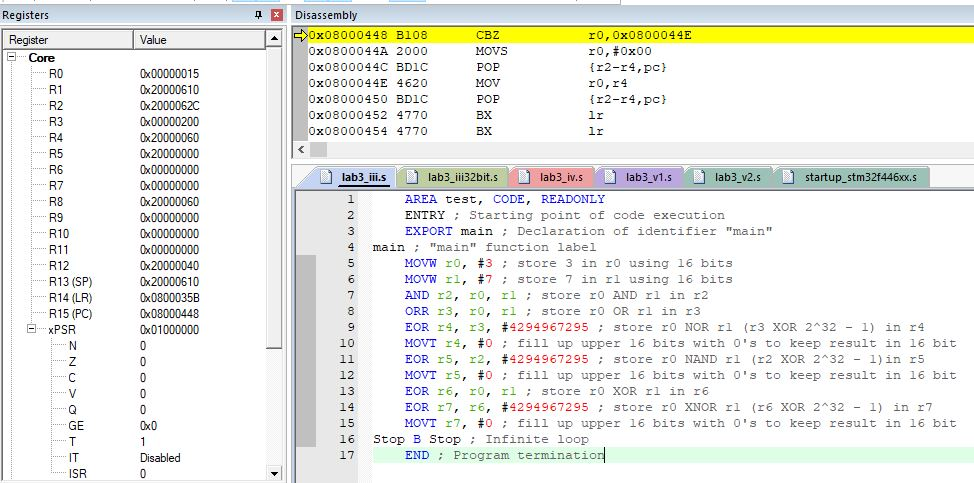
\includegraphics[scale=.7]{images/lab3_1_ss1.jpg}
    \caption{The system state after loading the code(for 16 bits) with status registers shown}
    \label{fig:before_task_three_one}
\end{figure}
\pagebreak
\subsection{Screenshot of the System State after Code Execution:}
\begin{figure}[ht]
    \centering
    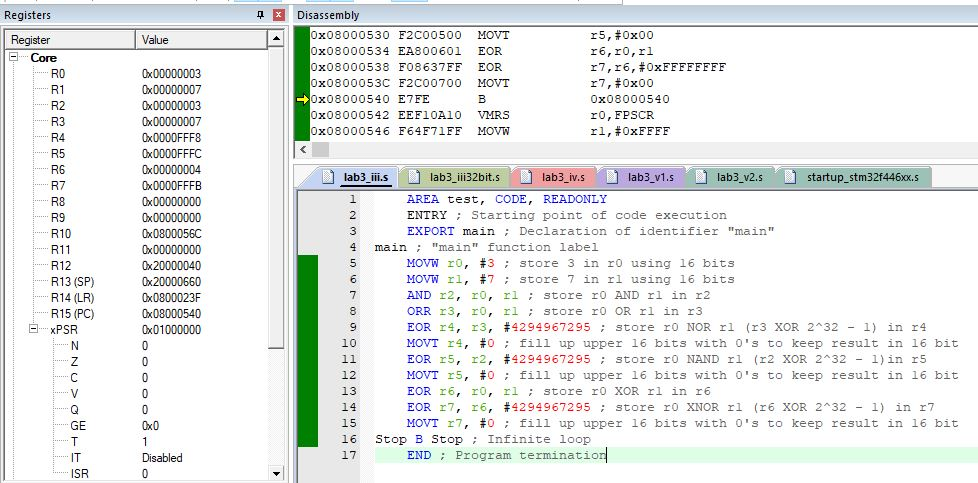
\includegraphics[scale=.7]{images/lab3_1_ss2.jpg}
    \caption{The system state after executing the code(for 16 bits) with status registers shown}
    \label{fig:after_task_three_one}
\end{figure}
\pagebreak
\subsection{Screenshot of the System State after Loading the Code:}
\begin{figure}[ht]
    \centering
    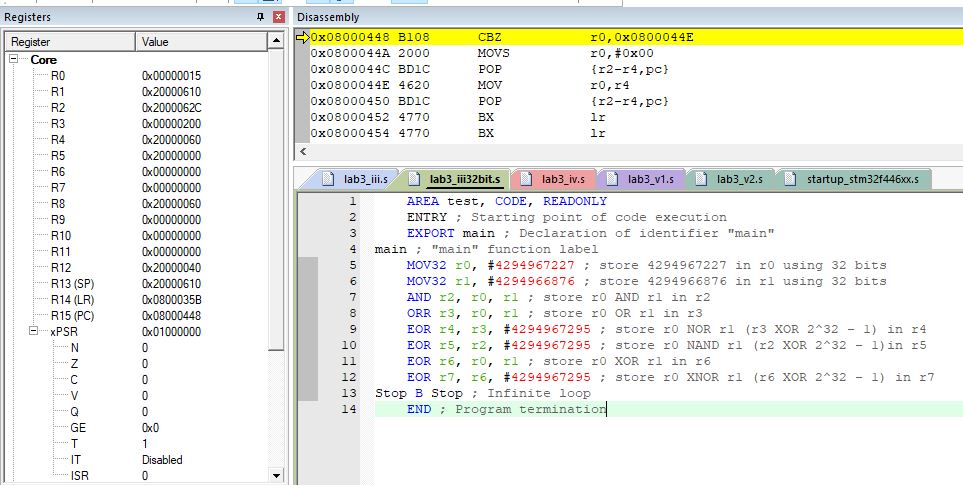
\includegraphics[scale=.7]{images/lab3_1_ss3.jpg}
    \caption{The system state after loading the code(for 32 bits) with status registers shown}
    \label{fig:before_task_three_two}
\end{figure}
\pagebreak
\subsection{Screenshot of the System State after Code Execution:}
\begin{figure}[ht]
    \centering
    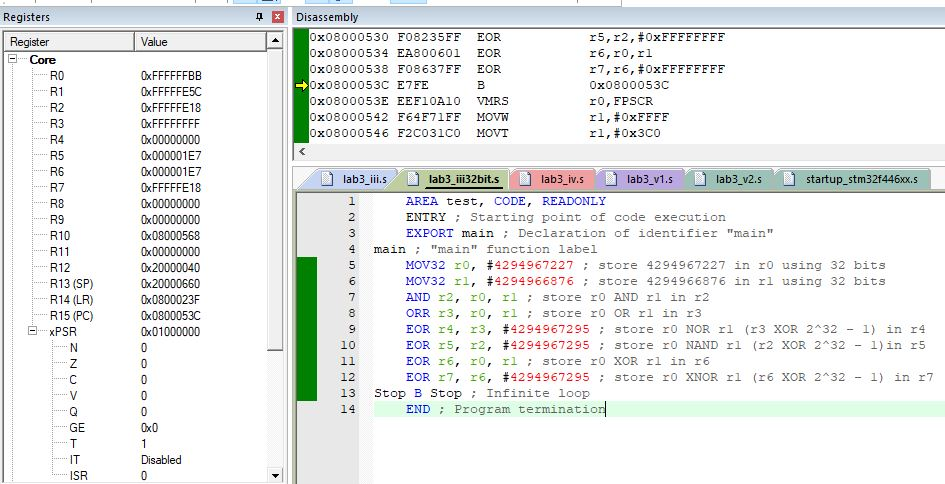
\includegraphics[scale=.7]{images/lab3_1_ss4.jpg}
    \caption{The system state after executing the code(for 32 bits) with status registers shown}
    \label{fig:after_task_three_two}
\end{figure}
\pagebreak
\section{Task iv}
\subsection{Explanation of Code:}
Shifting a number left and right is equivalent to multiplying and dividing it by a power of two, respectively. Logical and arithmetic shifts have the same function, except that arithmetic shift copies the sign bit into the vacated bit positions on the left.
\subsection{Description of Instructions:}
\textbf{MOV32} \\ The \verb|MOV32| instruction loads a register with either a 32-bit immediate value or any address.\\
\verb|MOVT{cond} Rd, #imm16|\\
\textbf{LSR}\\
\verb|LSR| provides the unsigned value of a register divided by a variable power of two, inserting zeros into the vacated bit positions.
\verb|LSR{S}{cond} Rd, Rm, Rs|\\
\verb|LSR{S}{cond} Rd, Rm, #sh|\\
\textbf{ASR}\\
\verb|ASR| provides the signed value of the contents of a register divided by a power of two. It copies the sign bit into vacated bit positions on the left.
\verb|ASR{S}{cond} Rd, Rm, Rs|\\
\verb|ASR{S}{cond} Rd, Rm, #sh|\\
\textbf{LSL}\\
\verb|LSL| provides the value of a register multiplied by a power of two, inserting zeros into the vacated bit positions.
\verb|LSL{S}{cond} Rd, Rm, Rs|\\
\verb|LSL{S}{cond} Rd, Rm, #sh|\\
\pagebreak
\subsection{Screenshot of the System State after Loading the Code:}
\begin{figure}[ht]
    \centering
    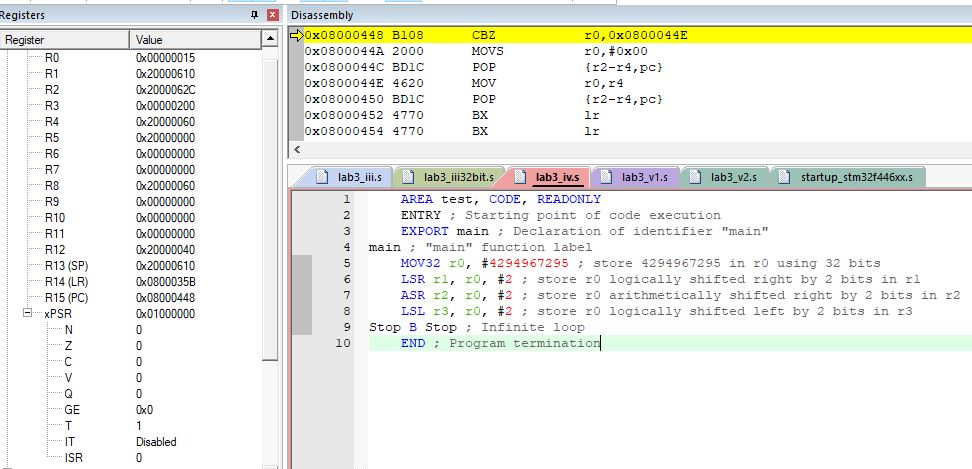
\includegraphics[scale=.7]{images/lab3_2_ss1.jpg}
    \caption{The system state after loading the code with status registers shown}
    \label{fig:before_task_four}
\end{figure}
\pagebreak
\subsection{Screenshot of the System State after Code Execution:}
\begin{figure}[ht]
    \centering
    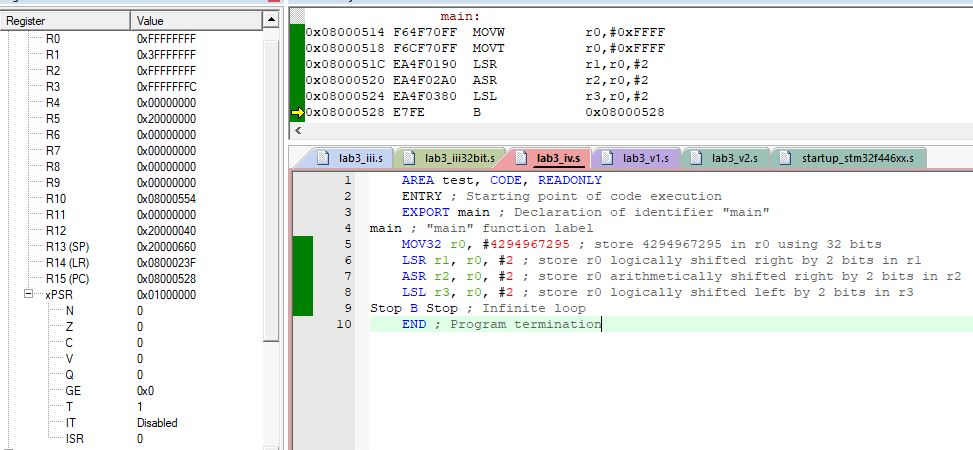
\includegraphics[scale=.7]{images/lab3_2_ss2.jpg}
    \caption{The system state after executing the code with status registers shown}
    \label{fig:after_task_four}
\end{figure}
\pagebreak
\section{Task 5}
\subsection{Explanation of Code:}
For addition, subtraction and multiplication, the \verb|ADD|, \verb|SUB| and \verb|MUL| instructions have been used to store the results of arithmetic operations of two registers in other registers.\\
In case of unsigned multiplications, UMULL instruction has been used.\\
\subsection{Description of Instructions:}
\textbf{ADD}\\
The \verb|ADD| instruction adds the values in Rn and Operand2 or imm12. \verb|S| is an optional suffix. If \verb|S| is specified, the condition flags are updated on the result of the operation.\\
\verb|ADD{S}{cond} {Rd}, Rn, Operand2|\\
\textbf{SUB}\\
The \verb|SUB|  instruction subtracts the value of Operand2 or imm12 from the value in Rn. If \verb|S| is specified, the condition flags are updated on the result of the operation.\\
\verb|SUB{S}{cond} {Rd}, Rn, Operand2|\\
\textbf{MUL}\\
The \verb|MUL| instruction multiplies the values from Rn and Rm, and places the least significant 32 bits of the result in Rd.\\
\verb|MUL{S}{cond} {Rd}, Rn, Rm|\\
\textbf{UMULL}\\
The \verb|UMULL| instruction interprets the values from Rn and Rm as unsigned integers. It multiplies these integers and places the least significant 32 bits of the result in \verb|RdLo|, and the most significant 32 bits of the result in \verb|RdHi|.\\
\verb|UMULL{S}{cond} RdLo, RdHi, Rn, Rm|\\
\textbf{MOVW}\\The \verb|MOVW| instruction only allows \#imm16 values to be loaded into the registers. \\
\textbf{MOV32} \\ The \verb|MOV32| instruction loads a register with either a 32-bit immediate value or any address.\\
\verb|MOVT{cond} Rd, #imm16|\\
\textbf{CMP}\\
The \verb|CMP| instruction subtracts the value of Operand2 from the value in Rn. This is the same as a \verb|SUBS| instruction, except that the result is discarded.\\
\verb|CMP{cond} Rn, Operand2|\\
\pagebreak
\subsection{Screenshot of the System State after Loading the Code:}
\begin{figure}[ht]
    \centering
    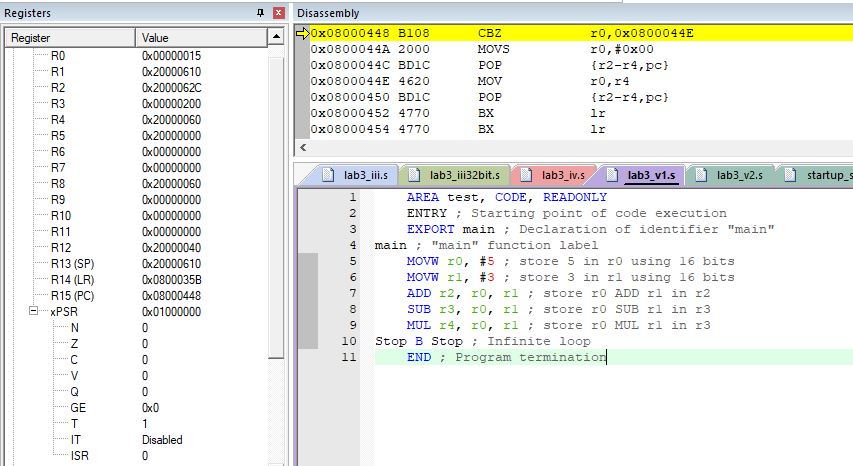
\includegraphics[scale=.7]{images/lab3_3_ss1.jpg}
    \caption{The system state after loading the code (restricting overflow) with status registers shown}
    \label{fig:before_task_five_one}
\end{figure}
\pagebreak
\subsection{Screenshot of the System State after Code Execution:}
\begin{figure}[ht]
    \centering
    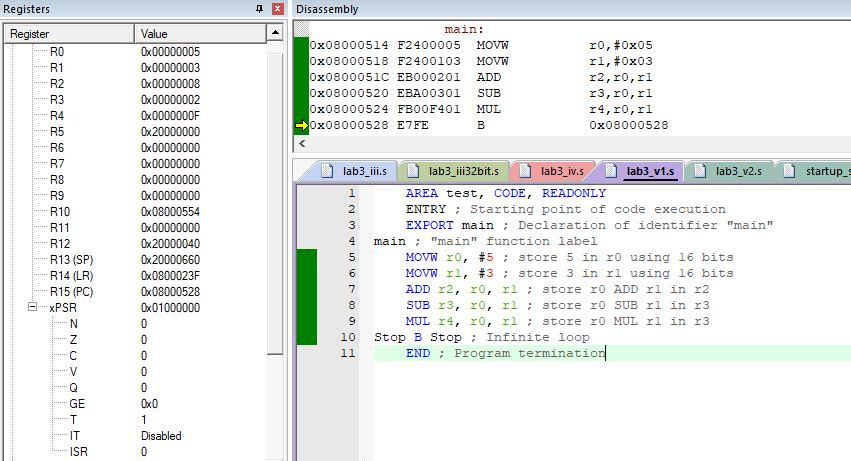
\includegraphics[scale=.7]{images/lab3_3_ss2.jpg}
    \caption{The system state after executing the code (restricting overflow) with status registers shown}
    \label{fig:after_task_five_one}
\end{figure}
\pagebreak
\subsection{Screenshot of the System State after Loading the Code:}
\begin{figure}[ht]
    \centering
    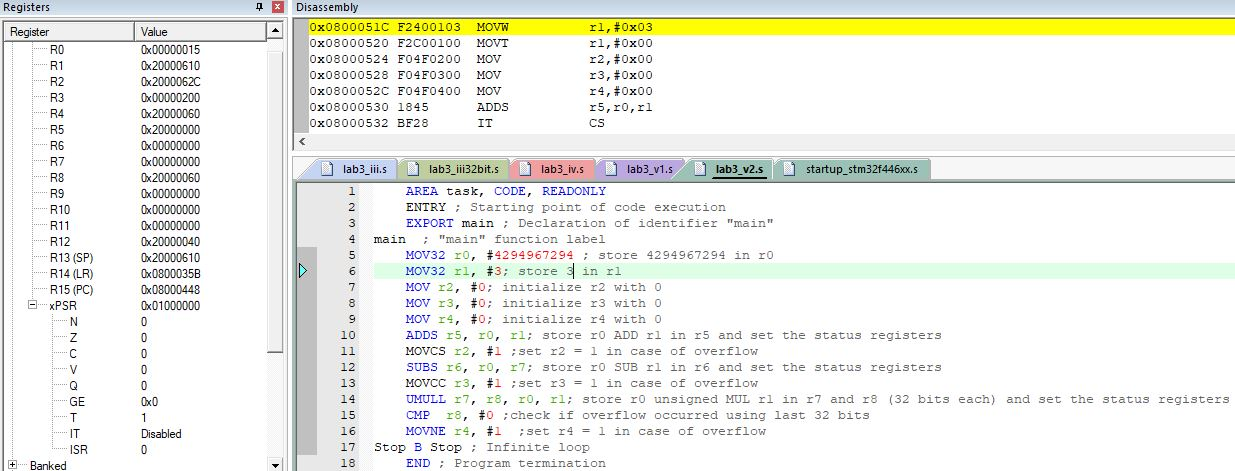
\includegraphics[scale=.6]{images/lab3_3_ss3.jpg}
    \caption{The system state after loading the code (handling overflow) with status registers shown}
    \label{fig:before_task_five_two}
\end{figure}
\pagebreak
\subsection{Screenshot of the System State after Code Execution:}
\begin{figure}[ht]
    \centering
    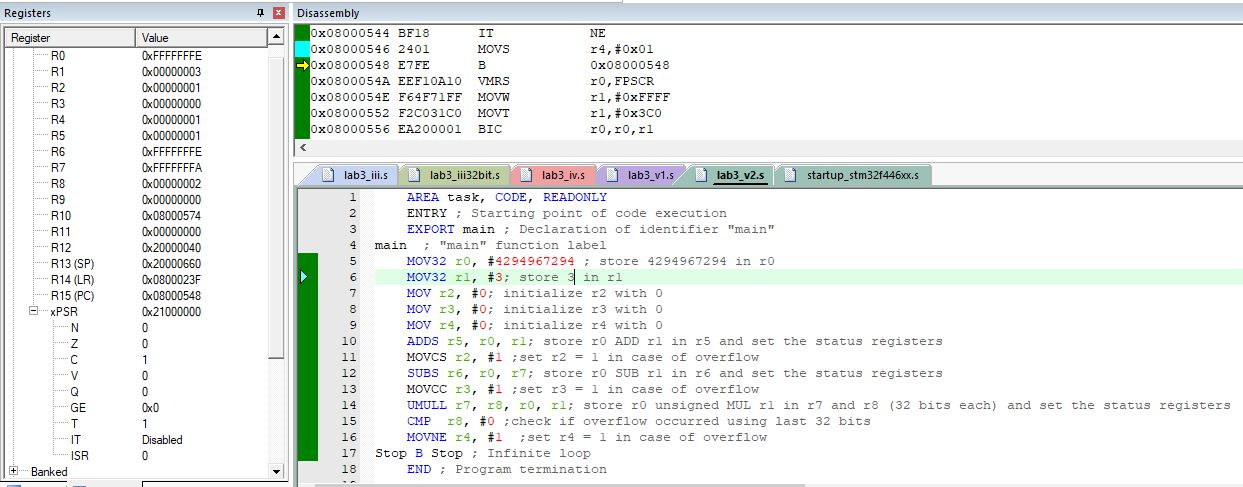
\includegraphics[scale=.6]{images/lab3_3_ss4.jpg}
    \caption{The system state after executing the code (handling overflow) with status registers shown}
    \label{fig:after_task_five_two}
\end{figure}
\end{document}
